\documentclass[UTF8,a4paper,12pt]{ctexart}
\usepackage[margin=2.5cm]{geometry}
\usepackage{graphicx}
\usepackage{booktabs}
\usepackage{float}
\usepackage{amsmath,amssymb}
\usepackage{caption}
\usepackage{setspace}
\usepackage{booktabs}


\pagestyle{plain}
\ctexset{
  section={format=\centering\heiti\bfseries\zihao{4},beforeskip=1.2ex,afterskip=1.0ex},
  subsection={format=\raggedright\heiti\bfseries\zihao{-4},beforeskip=1.0ex,afterskip=0.8ex},
  subsubsection={format=\raggedright\heiti\bfseries\zihao{-4},beforeskip=0.8ex,afterskip=0.6ex}
}
\setcounter{secnumdepth}{0}
\setlength{\parindent}{2em}
\setlength{\parskip}{0em}
\renewcommand{\baselinestretch}{1.0}
\graphicspath{{assets/}}

\begin{document}

\thispagestyle{empty}
\begin{center}
\vspace*{2.5cm}
{\heiti\zihao{2}2026吉林大学数学建模竞赛封面\par}
\vspace{2.2cm}
{\songti\zihao{4}\begin{tabular}{rl}
题目：& B题\\[0.8cm]
论文题目：& 城市极端降雨下内涝韧性提升与疏散路径优化\\[0.8cm]
提交编号：& \underline{\hspace{4cm}}\\[0.8cm]
\end{tabular}\par}
\vfill
\end{center}
\clearpage
\setcounter{page}{1}
\songti\zihao{-4}
\begin{center}
{\heiti\bfseries\zihao{3}城市极端降雨下内涝韧性提升与疏散路径优化\par}
\end{center}
\vspace{1em}
\section{摘要}
本文围绕城市极端短时强降雨条件下的内涝演化、韧性评价、动态疏散和综合改造问题展开研究。首先，结合降雨时序、路段基础信息和排水能力，建立路段积水深度动态递推模型，并通过最小二乘方法校准模型参数，进一步根据积水深度映射通行能力与安全度。其次，从抵御能力、恢复能力和适应能力三个维度构建内涝韧性评价体系，利用标准化加权评价和障碍度分析识别系统薄弱环节。再次，在积水深度随时间变化的约束下，建立兼顾疏散时间与路径安全度的动态路径优化方法。最后，针对管网改造、绿色设施建设等治理措施，构建以成本、韧性提升和积水消退时间为目标的综合优化模型，为城市内涝韧性提升提供定量决策依据。

{\heiti 关键词：}城市内涝；积水动态演化；韧性评价；动态疏散；多目标优化
\clearpage
\songti\zihao{-4}
\section{一、问题重述}

\subsection{1.1问题背景}

随着极端天气的出现次数增加，极端短时强降雨已经成为威胁现代城市安全的重大风险因素，我国北方城市近年来小时降雨量超过50mm的极端事件次数显著上升。因此分析并且评估不同降雨条件下不同路况的路段的积水深度、通行能力的动态变化规律，构建内涝韧性综合评价体系、安全疏散模型和综合治理优化方案，对提升城市防灾减灾能力、应急响应效率和在保障居民生命财产安全的领域具有重要的应用价值和实际意义。

\subsection{1.2问题重述}

问题一：要求根据路网基础信息、降雨时序数据等影响因素，建立城市路网积水动态演化模型在此基础上确定不同积水深度对应的路段的通行能力与安全程度。

问题二：要求从抵御、恢复、适应三个维度建立内涝韧性综合评价模型，识别内涝的薄弱环节。并且分析各个指标对内涝韧性的影响程度。最后给出薄弱路段与薄弱环节的识别结果。

问题三：要求以总疏散时间、路径安全度为评价目标，结合路段积水变化与通行能力通行规则与各个时段积水深度数据，设计可实时更新的疏散路径算法，并计算出起点到终点的最优动态路径与花费的时间和安全度。

问题四：要求以总成本最低、韧性提升最大、消退时间最短为目标，通过管网改造、绿色设施建设等方法，设计可以实施的内涝韧性提升综合改造方案，并对方案进行效果评估与鲁棒性分析。

\section{二、问题分析}

4该问题以城市短时强降雨引发的内涝治理为背景，在附表中给出了不同路况下各个路段的积水深度、通行能力等各项数据指标；和路网结构、排水设施等路况基础信息。我们通过在城市水文和交通运行的基本原理的基础建立城市内涝发生与演化的模型，从降雨、地表径流、管网排水、积水累积等多角度进行考虑，来评估内涝程度，判断应急疏散路线，解决题目给出的四个问题。我们需要已有的数据分析各路段积水深度随时间的动态演化规律、对系统内涝韧性进行综合评价、对极端降雨场景下动态安全疏散路径进行实时判断、对有限投入下内涝韧性提升的综合治理方案进行设计。

\subsection{2.1建立路网积水动态演化模型}

针对问题一，我们对片区各个路段分别分析积水深度和降雨时间、路段通行能力、积水深度之间的关系。通过对每个路段在不同时段的积水深度的变化的分析计算，发现积水深度随时间整体呈现先上升后下降的趋势，因此简单的线性模型无法对数据进行很好的拟合。因此为了能够对数据的变化趋势进行更加准确地描述，我们选择建立动态递推模型。基于最小二乘法，运用$MATLAB$中的$lsqnonlin$函数对该模型进行求解，得到各路段的模型参数，进而通过分析所得曲线的变化规律，得到各路段积水深度随时间的变化规律。

同时，我们对各路段在不同积水深度下的通行能力系数与安全度进行分析。通过应用附表3中给定的积水深度和通行能力的关系，可以看出积水深度超过一定阈值后，路段通行能力会迅速下降。因此，我们以附表3为依据，将各时段积水深度直接映射为通行能力系数与安全度，并引入残差校正项修正模型计算误差，得到路段通行状态数据。

\section{五、模型建立及求解}

\subsection{5.1问题一模型建立及求解}

\subsubsection{5.1.1动态递推模型的建立}

由问题一的分析，为了更好的拟合降雨时间与积水深度的关系，我们选择建立关于时间 \(t\) 的动态递推模型。

首先，将附表 2 中以 5 min 时间间隔的降雨数据合并为以 15 min 为时间间隔的积水时段。设附表 2 中第 $m$ 个 5 min 时段雨量为 \(r_m\)，第 $k$ 个 15 min 时段雨量为 \(R_k\)，则：

\[{{R}_{k}}=\sum_{m=3k-2}^{3k}{{r}_{m}},\quad \quad \quad \quad k=1,2,3,4\]

于是根据附表2可以得到四个时段的降雨总量为：

\[{{R}_{1}}=4+6+9=19,\quad \quad {{R}_{2}}=11+10+8=29,\]

\[{{R}_{3}}=6+4+2=12,\quad \quad {{R}_{4}}=2+1+1=4\]

根据城市排水工程标准中的思想，雨水产流量与降雨强度、径流系数和汇水面积等因素有关，表示为 \(Q=\psi\theta R\)。由于题目未给出完整汇水面积和管网水力参数，本文将路段产流过程简化为当前降雨贡献项和累计汇水贡献项。设 \(\psi_i\) 为第 \(i\) 条路段的路面径流系数，\(\theta_i\) 为当前降雨响应系数，\(\mu_i\) 为累计汇水响应系数，另设1 h内四个15 min时段雨量之和为 \(R_{\rm sum}\)，引入累计降雨比例 \(C_k=\sum_{j=1}^{k}R_j/R_{\rm sum}\)。则当前降雨造成的直接积水贡献为 \(P_{i,k}^{(1)}=\psi_i\theta_iR_k\)，累计降雨造成的滞后汇水贡献为 \(P_{i,k}^{(2)}=\psi_i\mu_iC_k\)。

上述三个参数中，\(\psi_i\) 由附表1中的路面类型直接确定，用来反映降雨转化为地表径流的比例。由于附表1中路面类型主要为沥青和水泥，且二者均为硬化路面，本文取沥青路面 \(\psi_i=0.95\)，水泥路面 \(\psi_i=0.90\)。\(\theta_i\) 表示当前时段降雨转化为积水的敏感程度，它主要受路段长度、最低标高、设计排水能力和地形坡度影响，即路段越长、标高越低、排水能力越弱或坡度越小，当前降雨越容易形成明显积水。\(\mu_i\) 表示累计降雨造成的滞后汇水效应，主要受最低标高、坡度、设计排水能力和路段长度影响。其中最低标高反映低洼汇水倾向，坡度和排水能力反映积水消退条件，路段长度反映潜在汇水尺度。因此，\(\theta_i\) 更强调当前降雨的即时产流影响，\(\mu_i\) 更强调前期降雨在低洼路段持续汇集和滞留的影响。

同时，路段积水具有一定延续性。设 \(h_i(k-1)\) 为第 \(i\) 条路段在上一时段末的积水深度，\(\rho_i\) 为该路段的滞蓄系数，则上一时段积水在当前时段的保留量为 \(B_{i,k}=\rho_i h_i(k-1)\)，其中 \(0\leq\rho_i\leq1\)。初始时刻认为路面尚未形成积水，即 \(h_i(0)=0\)。

另一方面，管网排水、道路坡度排泄等会削减路面积水。设 \(\delta_i\) 为第 \(i\) 条路段在一个15 min时段内的等效排水削减量，则排水削减项可记为 \(D_{i,k}=\delta_i\)。其中，\(\delta_i\) 结合附表1中设计排水能力、地形坡度和最低标高等因素进行解释，并通过附表4的积水深度数据校准得到。

参考 \(SWMM\) 模型中的水量平衡思想，路段积水变化可理解为“上一时段积水保留 + 本时段降雨输入 + 累计汇水输入 - 排水削减”。考虑到积水深度不能为负，得到残差校正前的基础动态递推模型：
\[
h_i^{(0)}(k)=
\max\left\{
0,\,
\rho_i h_i(k-1)
+\psi_i\left(\theta_iR_k+\mu_iC_k\right)
-\delta_i
\right\}.
\]

由于附表1未反映道路实际情况的细节因素，基础模型仍可能存在系统偏差。为提高模型对附表4观测数据的拟合能力，进一步引入路段固定偏差 \(u_i\) 和时段固定偏差 \(v_k\)。其中，\(u_i\) 用于修正不同路段长期偏高或偏低的误差，\(v_k\) 用于修正某一时段整体偏高或偏低的误差。于是校正后的积水深度为
\[
h_i(k)=
\max\left\{
0,\,
h_i^{(0)}(k)+u_i+v_k
\right\}.
\]

\subsubsection{5.1.2动态递推模型求解}

为了得到所建立模型中的参数，本文以附表4给出的实测积水深度作为校准依据，采用多起点约束非线性最小二乘法进行参数估计，并利用 $MATLAB$ 中的 $lsqnonlin$ 函数进行求解。

首先，根据附表4整理出8条路段在15 min、30 min、45 min和60 min四个时刻的观测积水深度矩阵：

\[
H=\{H_i(k)\}_{8\times 4}.
\]

其中，\(i=1,2,\ldots,8\) 表示路段编号，\(k=1,2,3,4\) 表示计算时段。再由附表2计算各时段降雨量 \(R_k\) 和累计降雨比例 \(C_k\)，作为外部输入。

基础模型中，每条路段需要估计滞蓄系数 \(\rho_i\)、当前降雨响应系数 \(\theta_i\)、累计汇水响应系数 \(\mu_i\) 和等效排水削减量 \(\delta_i\)。因此，待估参数向量可写为
\[
p=(\rho_1,\ldots,\rho_8,\theta_1,\ldots,\theta_8,
\mu_1,\ldots,\mu_8,\delta_1,\ldots,\delta_8).
\]

为保证参数具有合理的物理意义，设置约束条件为
\[
0\leq \rho_i\leq 0.99,\qquad
\theta_i\geq 0,\qquad
\mu_i\geq 0,\qquad
\delta_i\geq 0.
\]
其中，\(\rho_i\) 小于1表示在没有新增降雨时积水不会无限累积，其余参数非负表示降雨输入和排水削减的作用方向符合实际。

对于给定参数向量 \(p\)，先按照前文模型公式计算基础模型积水深度 \(h_i^{(0)}(k;p)\)，再与附表4中的观测值 \(H_i(k)\) 比较，得到残差
\[
e_i(k;p)=h_i^{(0)}(k;p)-H_i(k).
\]
将所有路段和所有时刻的残差展开为向量 \(e(p)\)，则参数估计问题可写为
\[
p^\ast=\arg\min_p \|e(p)\|_2^2
=\arg\min_p\sum_{i=1}^{8}\sum_{k=1}^{4}
\left[h_i^{(0)}(k;p)-H_i(k)\right]^2.
\]

在 $MATLAB$ 中，本文将残差矩阵展开为32维残差向量，并调用 $lsqnonlin$ 进行约束非线性最小二乘求解。由于模型中含有递推项，目标函数是非线性的，单一初值可能导致局部最优。因此，本文采用多起点搜索策略：先根据15 min时刻的观测积水深度给出一组初始响应系数，再设置若干扰动初值和随机初值；对每组初值分别调用 $lsqnonlin$，最后选择残差平方和最小的一组参数作为基础模型参数。

具体而言，初始滞蓄系数取 \(\rho_i^{(0)}=0.5\)，当前降雨响应系数根据初始时刻观测值近似反推为 \(\theta_i^{(0)}=H_i(1)/(\psi_iR_1)\)，累计汇水响应系数和等效排水削减量初值取 \(\mu_i^{(0)}=0,\delta_i^{(0)}=0\)。在此基础上增加多组扰动，以提高求解稳定性。$lsqnonlin$ 每次求解后返回残差平方和 $resnorm$，本文选择 $resnorm$ 最小的结果作为最优基础参数。

得到基础模型参数后，计算基础预测值与观测值之间的系统残差。考虑到基础模型可能存在路段层面和时段层面的固定偏差，进一步令
\[
H_i(k)-h_i^{(0)}(k)\approx u_i+v_k,
\]
其中 \(u_i\) 为路段固定偏差，\(v_k\) 为时段固定偏差。将该式写成线性最小二乘形式 \(r=Xc\)，其中 \(c=(u_1,\ldots,u_8,v_1,\ldots,v_4)^T\)。求解得到 \(u_i\) 和 \(v_k\)，并代入校正公式得到最终积水深度 \(h_i(k)\)。

为评价模型拟合效果，本文计算基础模型和残差校正后模型的误差指标。共有 \(N=32\) 个观测点，则
\[
RMSE=\sqrt{\frac{1}{N}\sum_{i=1}^{8}\sum_{k=1}^{4}
\left[h_i(k)-H_i(k)\right]^2},
\]
\[
MAE=\frac{1}{N}\sum_{i=1}^{8}\sum_{k=1}^{4}
\left|h_i(k)-H_i(k)\right|,
\]
\[
R^2=1-\frac{\sum_{i=1}^{8}\sum_{k=1}^{4}
\left[h_i(k)-H_i(k)\right]^2}
{\sum_{i=1}^{8}\sum_{k=1}^{4}\left[H_i(k)-\bar H\right]^2}.
\]
计算结果表明，基础动态模型的 \(RMSE=1.473\) cm，\(MAE=1.194\) cm，\(R^2=0.9550\)；加入路段偏差和时段偏差校正后，\(RMSE\) 降至 \(0.642\) cm，\(MAE\) 降至 \(0.508\) cm，\(R^2\) 提高到 \(0.9914\)。说明校正后的动态递推模型能够较好地拟合附表4中的积水深度变化，可用于后续通行能力和安全度评分计算。

需要说明的是，由于附表4仅包含8条路段在4个时刻的积水深度，共32个观测点，而模型中为不同路段设置了滞蓄系数、降雨响应系数、累计汇水响应系数和等效排水削减量，并进一步加入了路段偏差和时段偏差校正项，因此模型存在一定的过拟合风险。本文将该模型定位为主要用于本题场景下的积水状态估计和通行能力判断，不宜直接外推到其他城市片区或其他降雨过程。另一方面，基础动态模型在未加入残差校正时已经达到 \(R^2=0.9550\)，说明模型主体能够较好解释积水演化规律；残差校正主要用于消除路段和时段层面的系统偏差。因此，在本题给定数据范围内，校正后的结果具有较好的拟合精度和应用合理性。

根据上述模型求解结果，得到各路段在15 min、30 min、45 min和60 min时刻的积水深度，如表\ref{tab:q1-depth-result}所示。可以看出，各路段积水深度整体在45 min附近达到峰值，其中L5峰值积水深度达到31.63 cm，是最严重的积水路段。

\begin{table}[H]
\centering
\caption{各路段积水深度计算结果（单位：cm）}
\label{tab:q1-depth-result}
\begin{tabular}{ccccc}
\toprule
路段 & 15 min & 30 min & 45 min & 60 min \\
\midrule
L1 & 8.17 & 13.69 & 18.29 & 15.86 \\
L2 & 10.74 & 19.20 & 23.78 & 20.27 \\
L3 & 5.83 & 8.23 & 12.06 & 9.87 \\
L4 & 7.58 & 12.46 & 17.07 & 14.90 \\
L5 & 16.68 & 29.39 & 31.63 & 29.30 \\
L6 & 6.70 & 10.45 & 14.90 & 12.95 \\
L7 & 4.86 & 5.93 & 9.56 & 7.65 \\
L8 & 9.44 & 16.64 & 21.71 & 19.21 \\
\bottomrule
\end{tabular}
\end{table}

根据附表3中积水深度对应关系，将表\ref{tab:q1-depth-result}中的积水深度映射为通行能力系数与各路段安全度评分，结果如表\ref{tab:q1-capacity-result}和表\ref{tab:q1-safety-result}所示。当积水深度超过30 cm时，通行能力系数降为0，表示该路段完全中断。L5在45 min时安全度降为0，说明该时刻已不具备安全通行条件；L2和L8在45 min时安全度仅为0.2，也属于高风险路段。

\begin{table}[H]
\centering
\caption{各路段通行能力系数}
\label{tab:q1-capacity-result}
\begin{tabular}{ccccc}
\toprule
路段 & 15 min & 30 min & 45 min & 60 min \\
\midrule
L1 & 0.8 & 0.4 & 0.4 & 0.4 \\
L2 & 0.4 & 0.4 & 0.1 & 0.1 \\
L3 & 0.8 & 0.8 & 0.4 & 0.8 \\
L4 & 0.8 & 0.4 & 0.4 & 0.4 \\
L5 & 0.4 & 0.1 & 0.0 & 0.1 \\
L6 & 0.8 & 0.4 & 0.4 & 0.4 \\
L7 & 1.0 & 0.8 & 0.8 & 0.8 \\
L8 & 0.8 & 0.4 & 0.1 & 0.4 \\
\bottomrule
\end{tabular}
\end{table}

\begin{table}[H]
\centering
\caption{各路段安全度评分}
\label{tab:q1-safety-result}
\begin{tabular}{ccccc}
\toprule
路段 & 15 min & 30 min & 45 min & 60 min \\
\midrule
L1 & 0.9 & 0.6 & 0.6 & 0.6 \\
L2 & 0.6 & 0.6 & 0.2 & 0.2 \\
L3 & 0.9 & 0.9 & 0.6 & 0.9 \\
L4 & 0.9 & 0.6 & 0.6 & 0.6 \\
L5 & 0.6 & 0.2 & 0.0 & 0.2 \\
L6 & 0.9 & 0.6 & 0.6 & 0.6 \\
L7 & 1.0 & 0.9 & 0.9 & 0.9 \\
L8 & 0.9 & 0.6 & 0.2 & 0.6 \\
\bottomrule
\end{tabular}
\end{table}

综合积水深度、通行能力和安全度结果可知，L5为本片区最主要的内涝风险路段，在45 min时达到完全中断状态；L2和L8属于高风险路段，在降雨中后期通行能力显著下降；L7积水深度始终较低，是相对安全路段。上述结果将作为后续韧性评价和动态路径规划的基础。

为更直观地展示各路段积水深度随时间变化的规律，本文绘制了积水深度动态演化图，如图\ref{fig:q1-depth-evolution}所示。该图上半部分反映各路段积水深度随时间的变化趋势，下半部分用于比较同一时刻不同路段的积水差异。可以看出，各路段积水整体在45 min附近达到峰值，其中L5积水最为严重，L2和L8也表现出较高风险，L7整体积水较浅。

\begin{figure}[H]
\centering
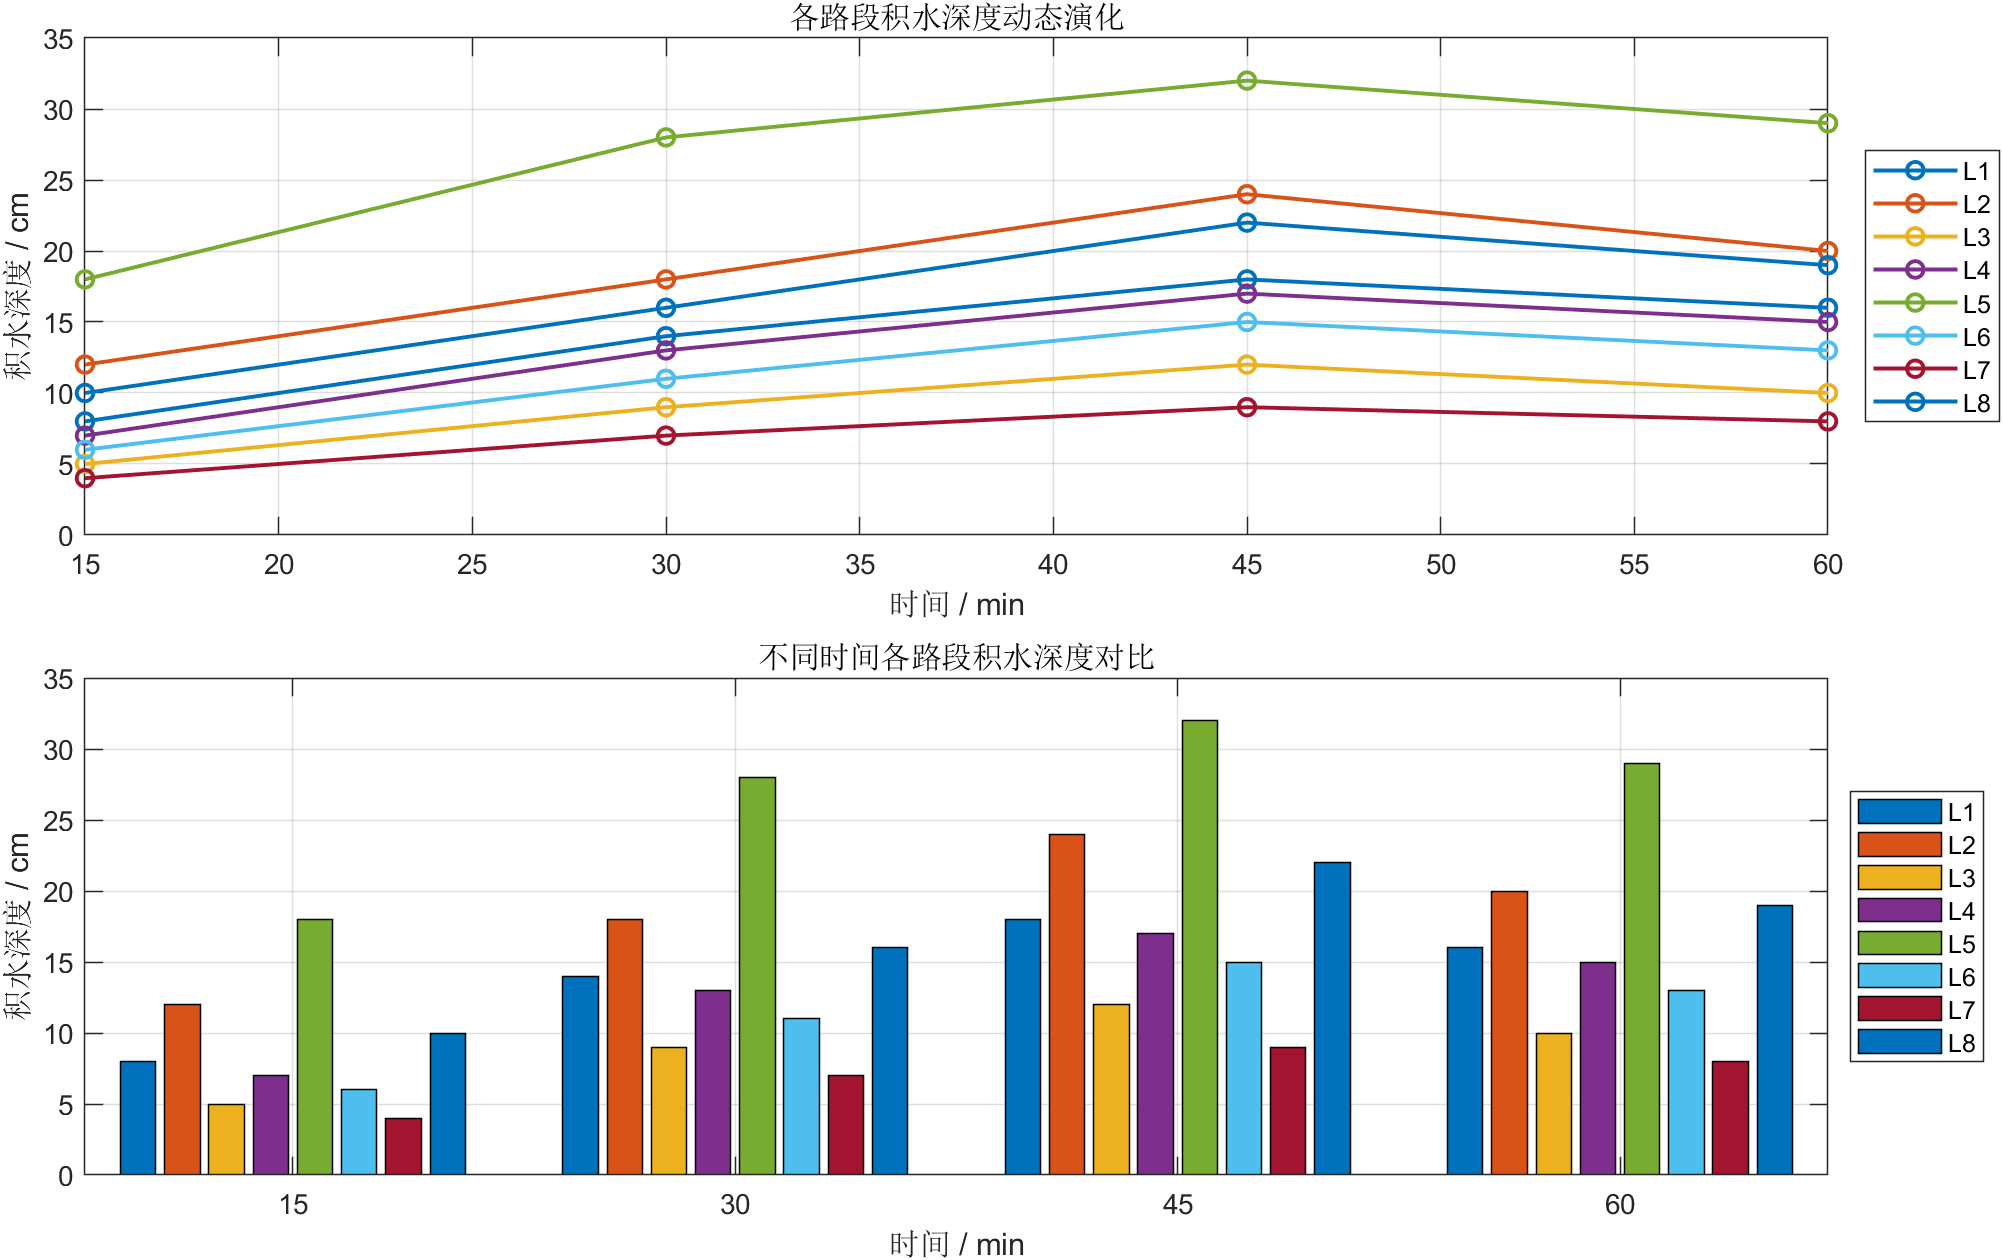
\includegraphics[width=0.92\linewidth]{q1_depth_evolution.png}
\caption{第一问各路段积水深度动态演化图}
\label{fig:q1-depth-evolution}
\end{figure}

积水深度热力图如图\ref{fig:q1-depth-heatmap}所示。热力图中颜色越深表示积水深度越大，
可以快速识别高风险路段和高风险时段。图中L5在45 min附近颜色最深，对应完全中断风险；
L2和L8在中后期颜色也较深，说明其通行能力明显下降。

\begin{figure}[H]
\centering
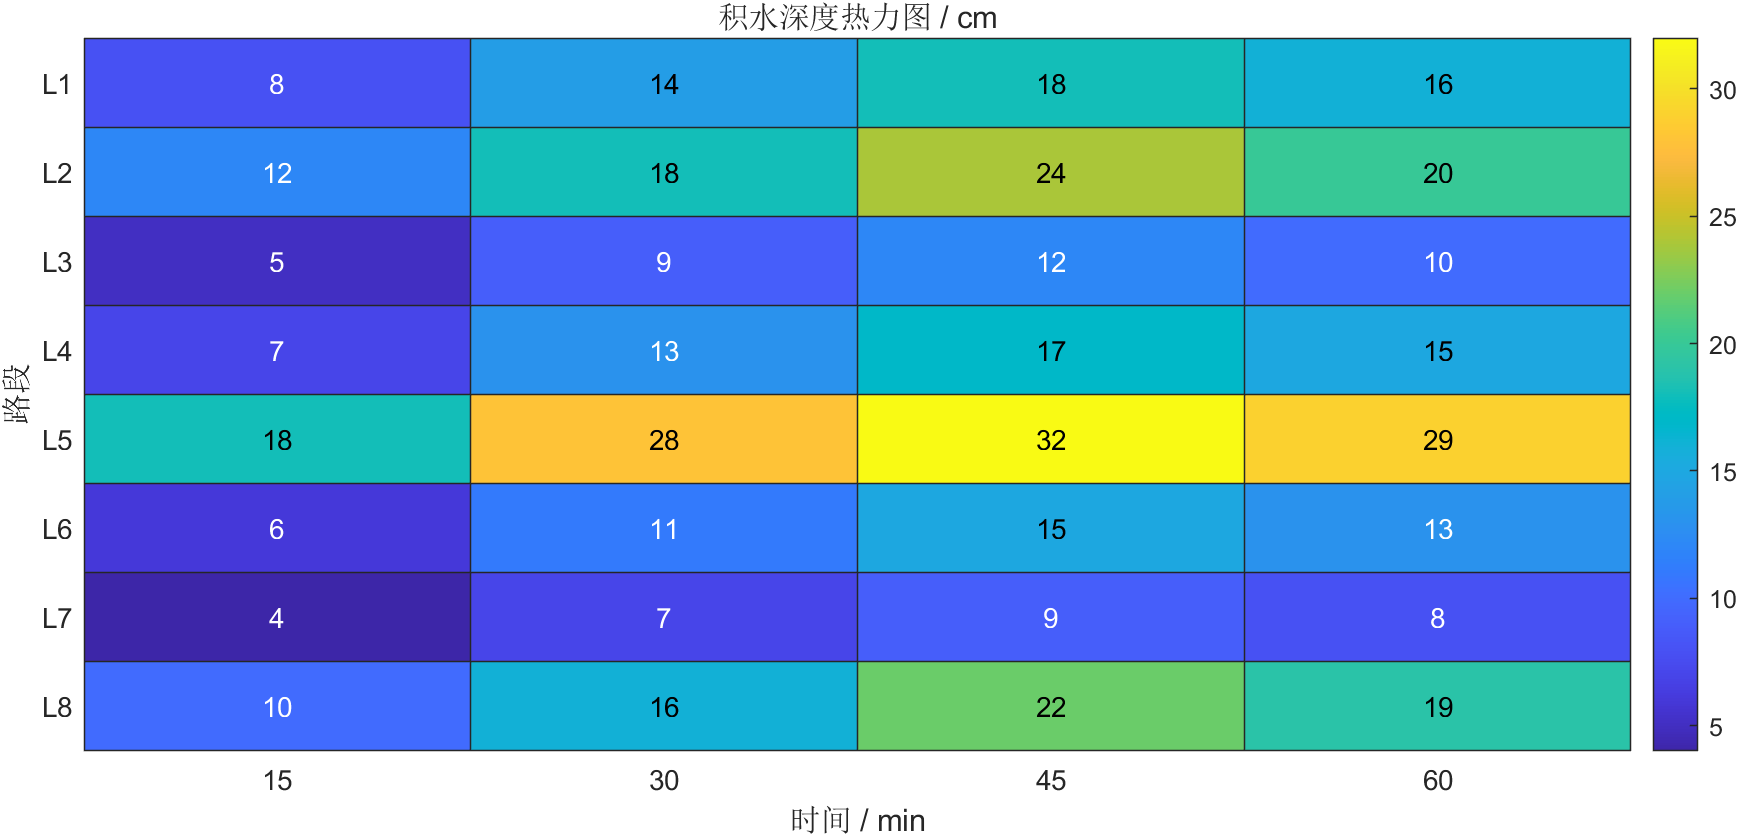
\includegraphics[width=0.78\linewidth]{q1_depth_heatmap.png}
\caption{第一问各路段积水深度热力图}
\label{fig:q1-depth-heatmap}
\end{figure}


\subsection{5.2 问题二模型的建立与求解}

\subsubsection{5.2.1基于标准化加权评价的综合韧性模型建立}

附表5已经给出了各二级指标的权重，因此本问不再重新确定权重，而是利用题目给定权重建立综合评价模型。由于各指标的量纲和含义不同，例如路网连通度、排水能力达标率为百分比指标，积水消退半衰期和应急响应时间为时间指标，绿色调蓄容积为体积指标，不能直接进行加权求和。因此，首先需要对各指标进行无量纲化处理，将其统一转化为 \(0\sim1\) 区间内的标准化得分。

设第 \(j\) 个二级指标的现状值为 \(x_j\)，理想满分值为 \(x_j^*\)，题目给定权重为 \(w_j\)，标准化得分为 \(s_j\)，其中 \(j=1,2,\cdots,9\)，且满足
\[
\sum_{j=1}^{9}w_j=1.
\]

对于路网连通度、排水能力达标率、抢修覆盖效率、绿色调蓄容积、预警覆盖率、疏散点位密度等正向指标，指标值越大表示韧性水平越高，采用如下标准化方式：
\[
s_j=\min\left\{\frac{x_j}{x_j^*},1\right\}.
\]

对于积水消退半衰期、应急响应时间等逆向指标，指标值越小表示韧性水平越高，因此采用理想值与现状值的比值进行标准化：
\[
s_j=\min\left\{\frac{x_j^*}{x_j},1\right\}.
\]

低洼路段占比同样属于逆向指标，但其理想满分值为0，若直接采用比值会出现分母为0的问题。因此，本文将其转化为非低洼路段比例：
\[
s_j=1-\frac{x_j}{100}.
\]

完成标准化后，建立片区综合韧性得分模型：
\[
R=100\sum_{j=1}^{9}w_js_j .
\]

其中，\(R\) 为研究片区综合韧性得分。\(R\) 越接近100，说明片区越接近理想韧性状态；\(R\) 越低，说明片区在抵御、恢复或适应能力方面存在越明显短板。

\subsubsection{5.2.2综合韧性评价模型求解}

根据附表5中各指标的现状值、理想满分值和题目给定权重，代入上一节建立的标准化加权评价模型，得到抵御能力、恢复能力和适应能力三个一级指标的综合评价结果，如表\ref{tab:q2-level-score}所示。

\begin{table}[H]
\centering
\caption{综合韧性评价结果}
\label{tab:q2-level-score}
\begin{tabular}{lccc}
\toprule
一级指标 & 权重合计 & 加权贡献/分 & 一级标准化得分/分 \\
\midrule
抵御能力 & 0.35 & 25.08 & 71.66 \\
恢复能力 & 0.37 & 18.17 & 49.10 \\
适应能力 & 0.28 & 13.88 & 49.58 \\
\bottomrule
\end{tabular}
\end{table}

由表\ref{tab:q2-level-score} 可知，抵御能力得分为 71.66 分，明显高于恢复能力和适应能力，说明该片区在路网连通、排水能力和低洼路段控制方面具有一定基础。但恢复能力得分仅为 49.10 分，适应能力得分为 49.58 分，均处于较低水平，说明片区在积水消退、应急响应和疏散支撑等方面存在明显不足。

综合各二级指标得分，可得研究片区现状综合韧性得分为：

\[
R=100\sum_{j=1}^{9}w_js_j=57.13.
\]

若将韧性水平划分为“较强、中等、偏弱、较差”四个等级，则该片区现状韧性属于偏弱水平。该结果表明，在极端短时强降雨条件下，研究片区虽然具有一定抵御能力，但整体系统仍难以快速恢复，内涝发生后容易出现道路通行能力下降、积水消退缓慢和疏散压力增大的问题。

\subsubsection{5.2.3障碍度分析与薄弱环节识别}

为了进一步比较抵御能力、恢复能力和适应能力三个一级指标的相对水平，设第 \(g\) 个一级指标包含的二级指标集合为 \(\Omega_g\)，则该一级指标的标准化得分定义为：
\[
R_g=100\frac{\sum_{j\in\Omega_g}w_js_j}{\sum_{j\in\Omega_g}w_j}.
\]

该指标消除了不同一级指标权重合计不同带来的影响，可用于判断抵御能力、恢复能力和适应能力三个维度本身的强弱。

仅得到综合韧性得分还不能说明哪些指标对整体韧性影响最大。为识别系统薄弱环节，本文进一步引入障碍度模型。第 \(j\) 个指标相对于理想状态的偏离程度为 \(1-s_j\)，再结合该指标权重 \(w_j\)，定义指标障碍度为：
\[
D_j=\frac{w_j(1-s_j)}{\sum_{j=1}^{9}w_j(1-s_j)}.
\]

其中，\(D_j\) 表示第 \(j\) 个指标对整体韧性的障碍度。障碍度越大，说明该指标与理想状态差距越大，且其在综合评价中的权重越高，对整体韧性的拖累越明显。因此，可根据 \(D_j\) 的大小对薄弱环节进行排序。

为进一步分析各指标对整体韧性的影响程度，本文利用障碍度模型计算各二级指标对综合韧性得分的制约程度。障碍度越大，说明该指标与理想状态差距越大，且其权重较高，对整体韧性的拖累越明显。计算结果如表\ref{tab:q2-obstacle}所示。

\begin{table}[H]
\centering
\caption{主要薄弱指标障碍度排序}
\label{tab:q2-obstacle}
\begin{tabular}{lcc}
\toprule
二级指标 & 标准化得分 & 障碍度/\% \\
\midrule
积水消退半衰期 & 0.4444 & 19.44 \\
绿色调蓄容积 & 0.3429 & 16.86 \\
应急响应时间 & 0.4167 & 16.33 \\
疏散点位密度 & 0.4200 & 10.82 \\
排水能力达标率 & 0.6800 & 9.70 \\
\bottomrule
\end{tabular}
\end{table}

由表\ref{tab:q2-obstacle}可知，积水消退半衰期的障碍度最高，达到19.44\%，说明暴雨后积水消退速度慢是制约片区韧性的首要因素。
绿色调蓄容积和应急响应时间的障碍度分别为16.86\%
和16.33\%，表明片区在雨洪调蓄与应急处置方面仍存在明显短板。
疏散点位密度和排水能力达标率同样对整体韧性有较大影响，说明内涝发生后，居民疏散承载能力和管网排水能力仍需进一步提升。

因此，研究片区的薄弱环节可以概括为：恢复能力不足是首要短板，具体表现为积水消退半衰期较长、应急响应时间偏长；适应能力不足是次要短板，具体表现为绿色调蓄容积不足、疏散点位密度偏低；抵御能力中排水能力达标率仍有提升空间。

\subsubsection{5.2.4薄弱路段识别}

由于附表5反映的是片区整体韧性水平，不能直接给出具体薄弱路段。为识别路段层面的薄弱对象，本文结合第一问得到的各路段积水深度、通行能力和安全度，构造路段风险指数。设第 \(i\) 条路段的最大积水深度为 \(H_i^{\max}\)，所有路段中的最大积水深度为 \(H^{\max}\)，该路段平均通行能力和平均安全度分别为 \(\bar K_i\)、\(\bar S_i\)，则路段风险指数定义为：
\[
V_i=0.4\frac{H_i^{\max}}{H^{\max}}+0.3(1-\bar K_i)+0.3(1-\bar S_i).
\]

\(V_i\) 越大，说明该路段在内涝过程中的脆弱性越高，可据此识别薄弱路段。利用路段风险指数对L1至L8进行排序，结果如表\ref{tab:q2-road-risk}所示。

\begin{table}[H]
\centering
\caption{薄弱路段风险排序}
\label{tab:q2-road-risk}
\begin{tabular}{lcccc}
\toprule
路段 & 最大积水深度/cm & 平均通行能力 & 平均安全度 & 风险等级 \\
\midrule
L5 & 31.63 & 0.150 & 0.250 & 完全中断/极高风险 \\
L2 & 23.78 & 0.250 & 0.400 & 高风险 \\
L8 & 21.71 & 0.425 & 0.575 & 高风险 \\
L1 & 18.29 & 0.500 & 0.675 & 中风险 \\
L4 & 17.07 & 0.500 & 0.675 & 中风险 \\
\bottomrule
\end{tabular}
\end{table}

由表\ref{tab:q2-road-risk}可知，L5、L2和L8是研究片区内涝过程中的主要薄弱路段。其中L5最大积水深度达到31.63 cm，超过30 cm的完全中断阈值，平均通行能力和平均安全度均处于较低水平，是最优先治理的风险路段。L2和L8最大积水深度均超过20 cm，通行能力显著下降，属于高风险路段。

\subsection{5.3 问题三模型的建立与求解}
\subsubsection{5.3.1模型假设}
题目附表只给出了L1-L8的路段属性和逐时段积水深度，没有给出完整道路连接表。因此，本文在不违背附表数据的前提下，依据道路等级、最低标高和疏散逻辑构造典型路网结构。构造原则为：L1、L3、L6 为主干路，作为主要通行骨架；L2、L5、L8为次干路，连接主干路与中心低洼区；L5最低标高为 198.9 m，设为易涝路段；L7标高最高且最低积水风险最低，因此设置为通往疏散点的高地支路。

（有图）

\subsubsection{5.3.2建立动态边权模型}

根据第一问输出的每时段积水深度和附表3 的映射关系，可以得出每条路段在15、30、45、60 min的积水深度、通行能力系数和安全度评分。设路段自由流速度主干路为 40 km/h、次干路为 30 km/h、支路为 20 km/h。若第 i 条路段在时刻t的通行能力为\(K_i(t)\)，则实际通行时间为：
\[
T_i(t) = \frac{l_i}{v_i^0 K_i(t)}
\]
当\(K_i(t)\)=0时，路段完全中断，算法中删除该边。为同时考虑安全性，引入安全惩罚\(R_i(t)\)并计算综合边权\(C_i(t)\)其中本文取\(\omega\) = 0.5，\(\tau\)=3.0min，用于将安全惩罚折算为时间代价：
\[
R_i(t) = -\ln\left(\max\left\{S_i(t), \varepsilon\right\}\right)
\]

\[
C_i(t) = \omega T_i(t) + (1 - \omega)\tau R_i(t)
\]

\subsubsection{5.3.3动态边权模型求解与结果}
以居民区节点N0为起点、应急疏散点N6为终点，逐时段运行动态Dijkstra 算法，结果如下：

（有图）

借此我们可以对每个候选路径的可通行状况，花费总时间和安全度等指标进行估计

（有图）



\end{document}
